%%% Simulering af gain-fase for 2. iteration

\subsection{Spændingsdeler}
Simulering af spændingsdeleren ses på figur~\ref{fig:simulering_voltage_divider}. Her er der målt et gennemsnit af den spænding der ligger over $R_{FB2}$, og dermed den spænding der ligger på indgangen af fejlforstærkeren. Spændingen aflæses til $2.499V$, hvilket blev designet efter $2.5V$.


\begin{figure}[H]
	\center
	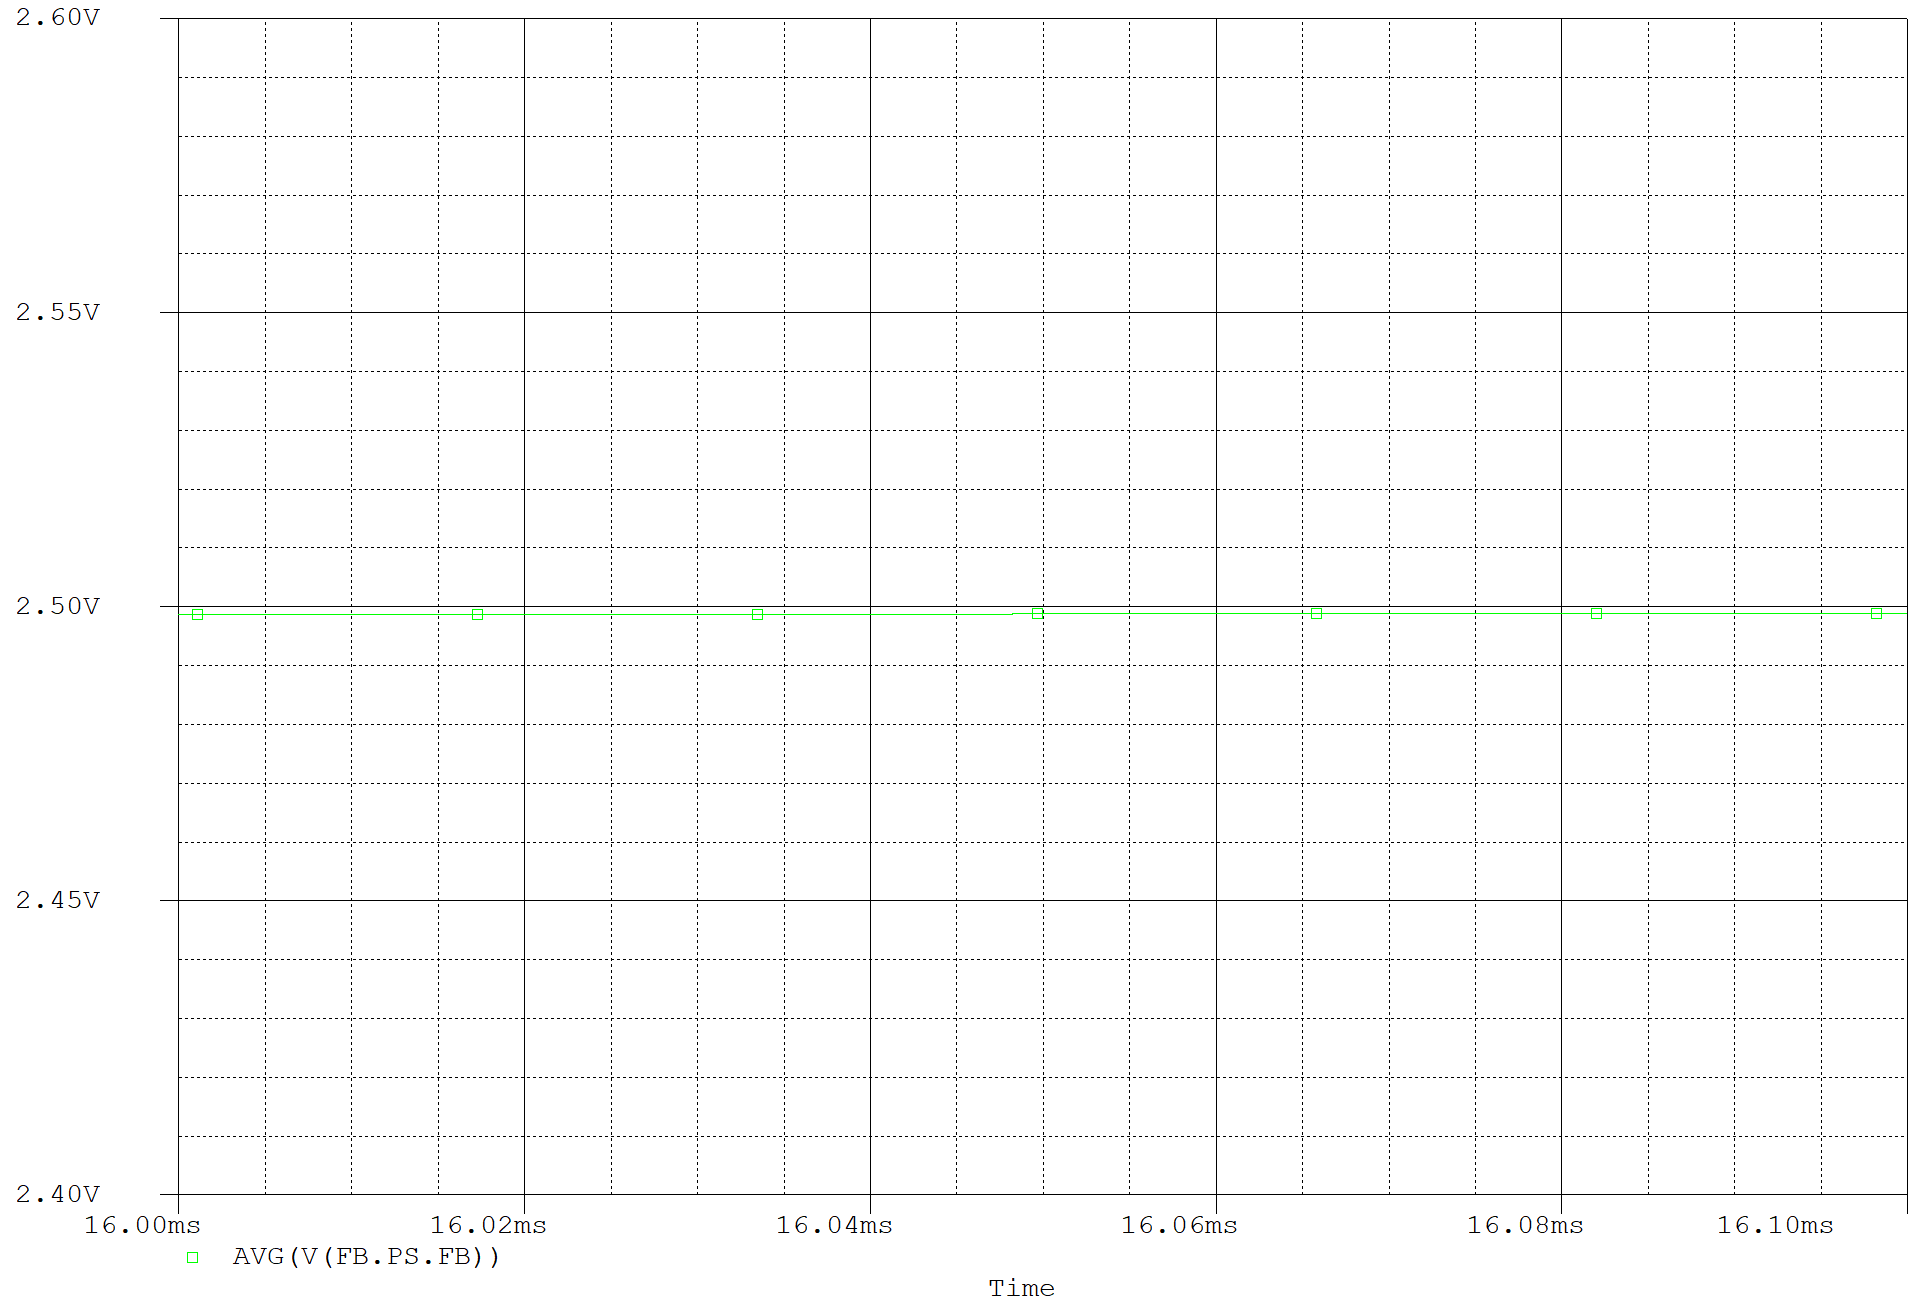
\includegraphics[max width=0.7\linewidth]{/tex/2iteration/billeder/Simulering_voltage_divider.png}
	\caption{Simulering spændingsdeler}
	\label{fig:simulering_voltage_divider}
\end{figure}


\subsection{Gain-fase}
Simuleringsdiagrammet for gain-fase, ses på figur~\ref{fig:sim_gain_fase_top}. For at lave simuleringen, indføres der et fejlsignal i tilbagekoblingen til fejlforstærkeren. Det gøres ved at indsætte en ekstra modstand inden spændingsdeleren, som ses på figur~\ref{fig:sim_gain_fase_2iteration}. Impedansen af denne modstand vælges til $51.1\ohm$, for at tilpasning til den network analyzer der bruges i realiseringen. Derudover vil modstanden ikke påvirke spændingsdeleren, da den er meget lille ift. $RFB1$. Da der indføres et fejlsignal på indgangen, mens ændringen på udgangen monitoreres, er det åbensløjfen der simuleres. 

\begin{figure}[H]
	\center
	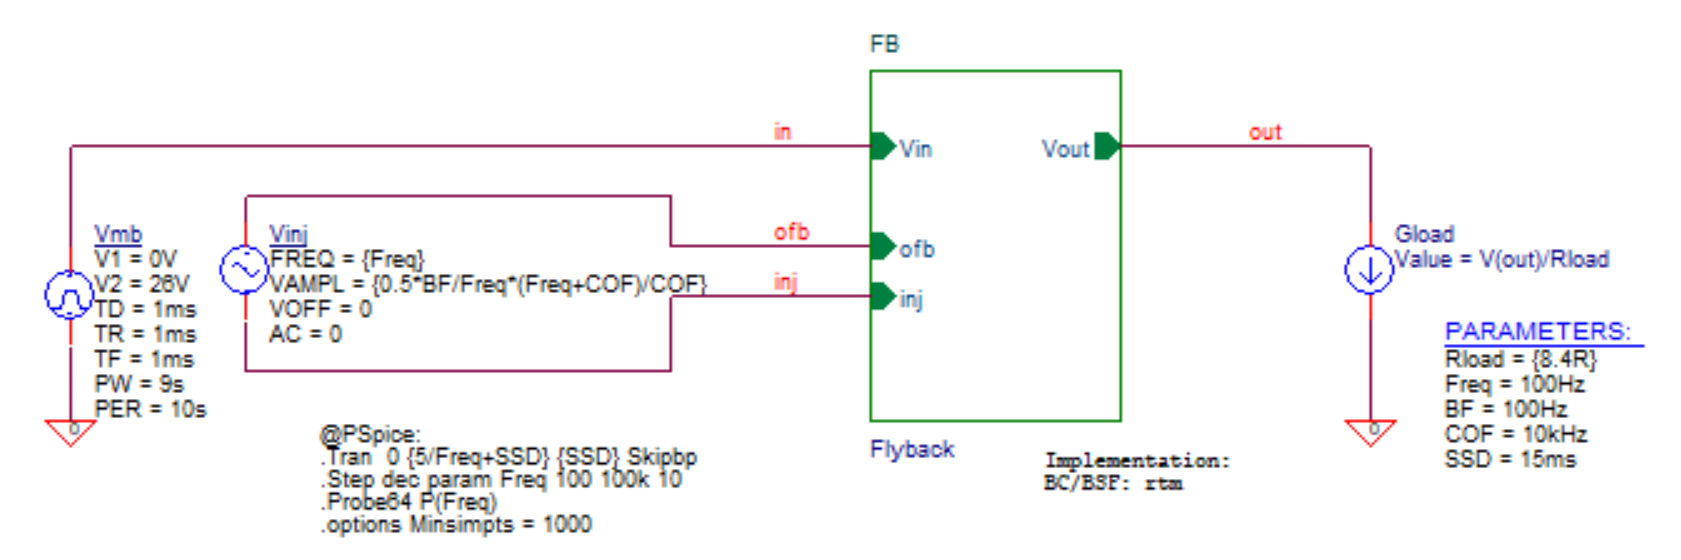
\includegraphics[max width=0.7\linewidth]{/tex/2iteration/billeder/Simulering_gain_fase_top.png}
	\caption{Gain-fase simuleringsdiagram}
	\label{fig:sim_gain_fase_top}
\end{figure}

\begin{figure}[H]
	\center
	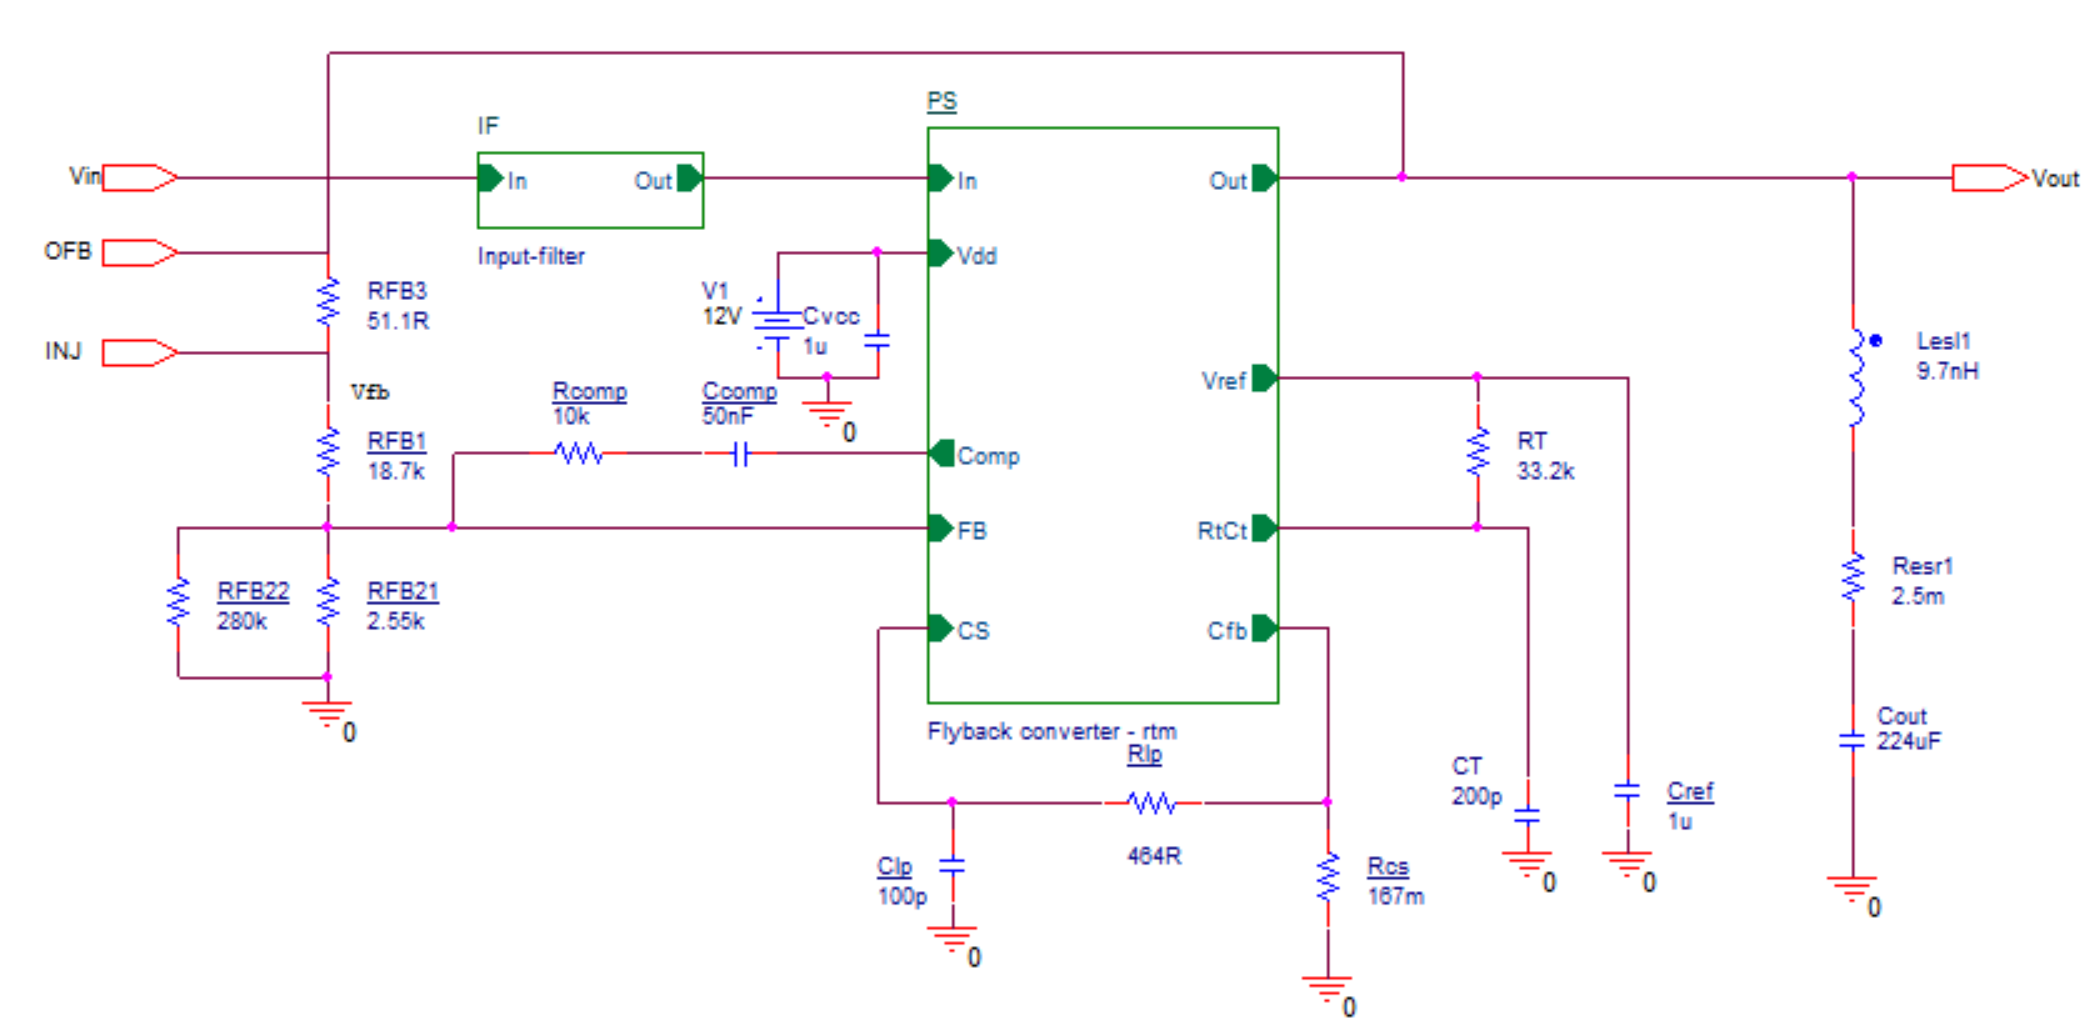
\includegraphics[max width=0.7\linewidth]{/tex/2iteration/billeder/Simulering_gain_fase_2iteration_flyback.png}
	\caption{Flyback blok - Gain-fase simulering}
	\label{fig:sim_gain_fase_2iteration}
\end{figure}

For at lave gain-fase simuleringen skal der foretages et frekvens-sweep af fejlsignalet. Derfor skal der laves en AC-simulering af kredsløbet. Det er dog ikke muligt med det bibliotek der bruges af UCC1801. Derfor foretages der en transient simulering, hvor frekvensen af fejlkilden løbende hæves. Dette giver en fil, med en simulering af alle ønskede frekvenser. Ud fra denne fil kan p-spice generere den tilhørende AC-fil, hvor gain-fase af systemet kan plottes. 

For at sætte simuleringen op i p-spice, indsættes tekstblokken \textit{@PSpice:}. Den ses på figur~\ref{fig:sim_gain_fase_top}. I den vælges længden på simuleringerne og frekvens-sweep'et. På første linje defineres længden af hver simulering. Den første og den sidste($0$ og $SSD$) del af linjen definerer opstarten, hvor $SSD=15ms$. Ved kommandoen \textit{Skipbp}, vælges det at se bort fra opstarten, og dermed kun se steady-state. Den midterste del af linjen($5/Freq+SSD$) definerer hvor langt selve signalet skal være. Hvor Freq er den variable frekvens. $5/Freq$ bestemmer at der simuleres fem perioder, og $+SSD$ tager højde for at opstarten ikke medtages. 

Anden linje definerer om der ønskes et lineært eller et logaritmisk sweep. Ved at bruge kommandoen \textit{dec}, for deacde, vælges et logaritmisk sweep. Derudover vælges start- og stopfrekvens, samt hvor mange simuleringer der skal foretages i hver dekade. Her vælges en startfrekvens på $100\hertz$, en slutfrekvens på $100k\hertz$, og 10 simuleringer per dekade. Da systemets dominerende pol ligger ved $132\hertz$, ville det være optimalt at have en startfrekvens på $10\hertz$. Dette var dog ikke muligt pga. simuleringstid og filstørrelse. De sidste to linjer fortæller p-spice, at det er Freq der er variabel. 

Opsætningen af indgangskilden og udgangsloaden, gøres på samme måde som ved Constant Load. Amplituden af fejlkilden, opsættes således amplituden falder når frekvensen stiger. Dette sikrer at systemet ikke overstyres ved høje frekvenser. Samtidig sikres på den måde at have en lidt højere amplitude ved de lavere frekvenser. Det hjælper til signalstøjforholdet, som er mest kritisk ved de lavere frekvenser, da gain her er høj\cite{evalgp}.

Simulering af gain-fase for selve power modulet er vist på figur~\ref{fig:sim_gain_fase_power}. Her er gain grøn og fasen er rød. Der er målt mellem udgangen af fejlforstærkeren og udgangen af converteren. Det ses at når frekvensen nærmer sig $10k\hertz$, bliver simuleringen usikker. Derfor vil det primært være analysen der bruges til sammenligning med realiseringen. Båndbredden kan dog aflæses til ca. $1200\hertz$, hvilket stemmer nogenlunde overens med analysen, som blev aflæst til ca. $1430\hertz$. Derudover aflæses gain ved en frekvens på $100\hertz$ til ca. $17.4\decibel$. Ved analysen blev dette aflæst til ca. $18\decibel$. Ud fra disse punkter kan det ses at simulering passer nogenlunde ved de lavere frekvenser. 

\begin{figure}[H]
	\center
	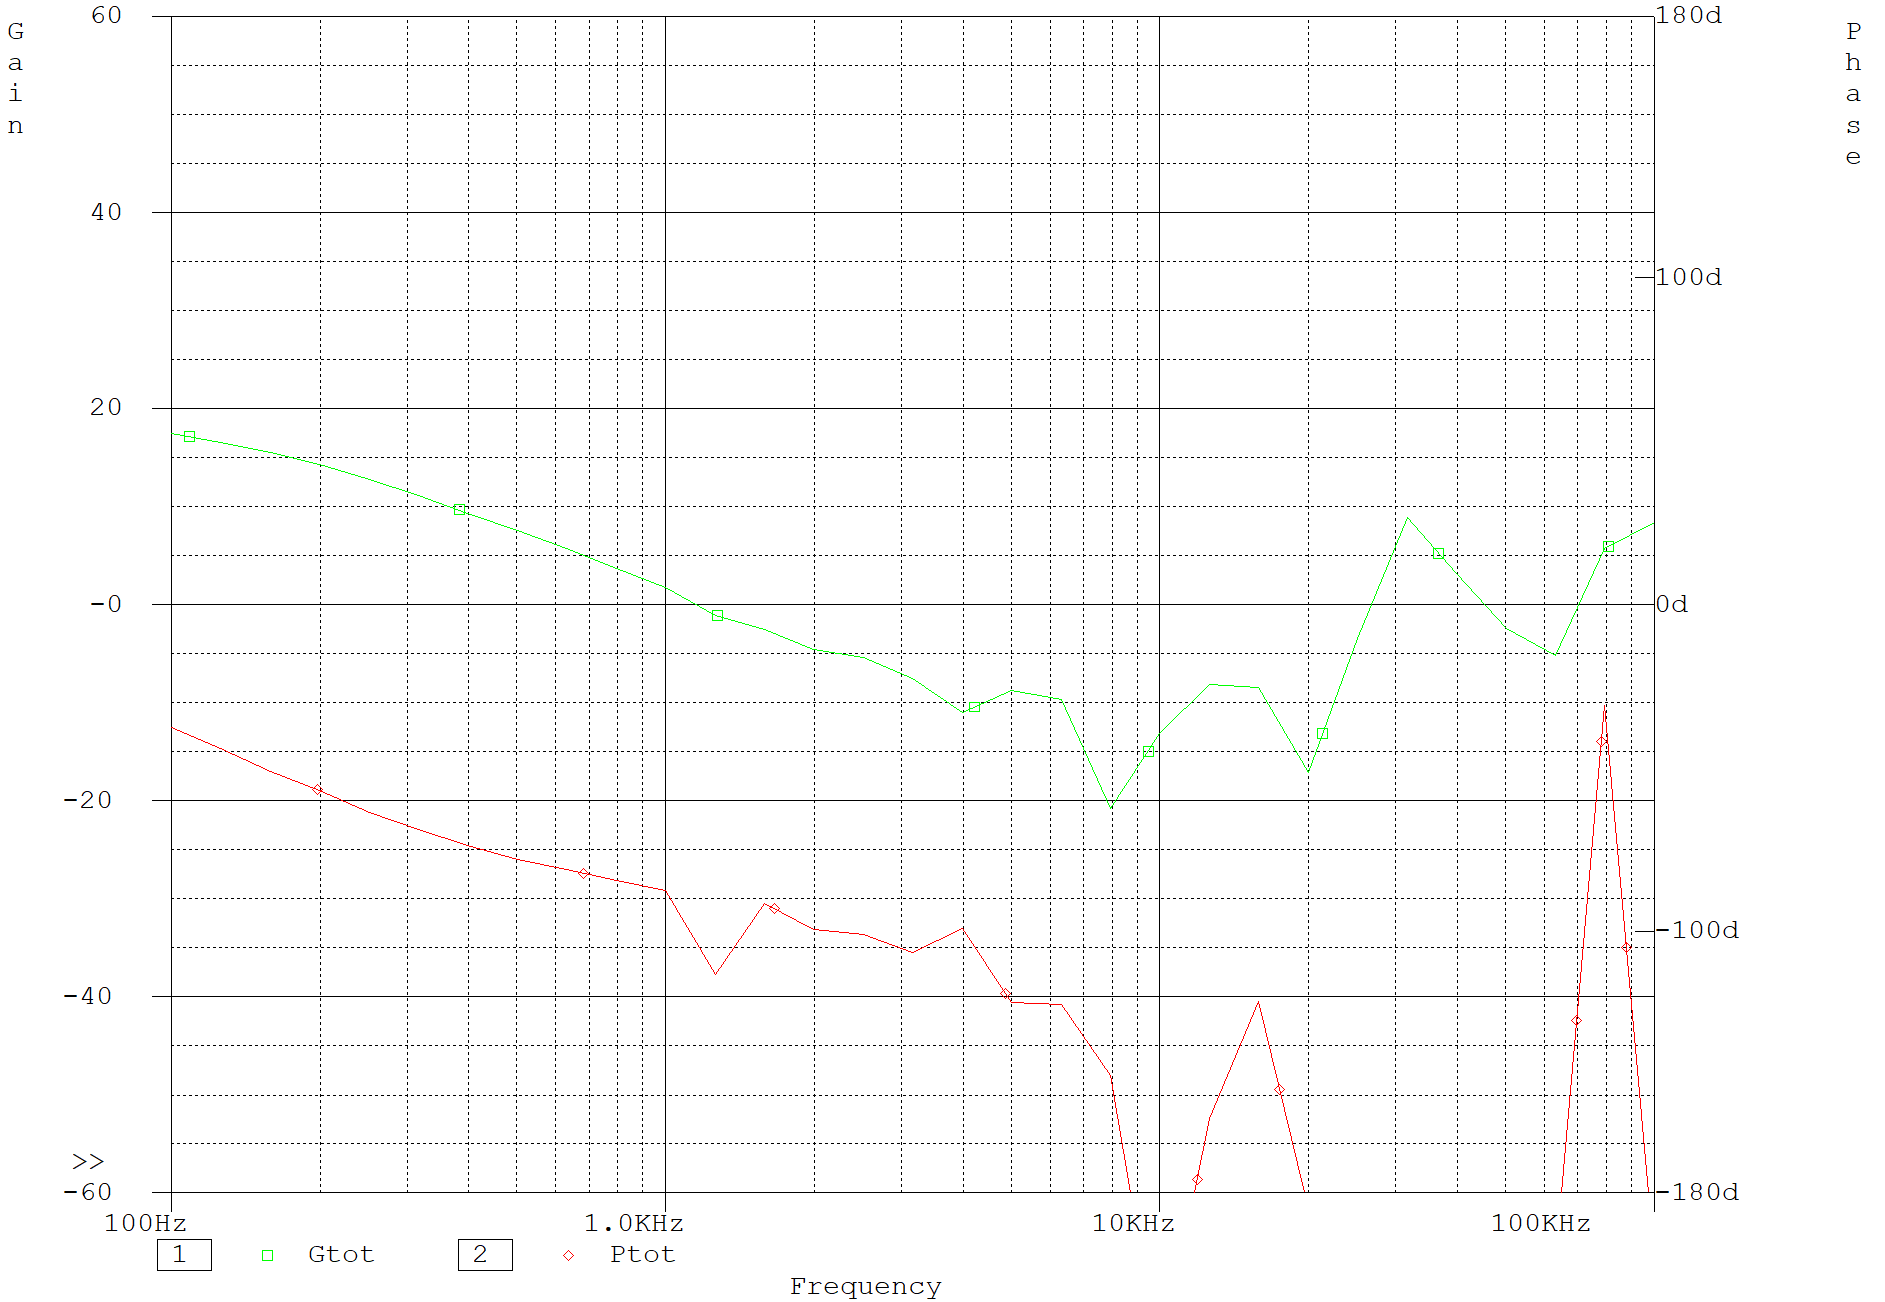
\includegraphics[max width=0.7\linewidth]{/tex/2iteration/billeder/Simulering_gain_fase_power.png}
	\caption{Gain-fase simulering for power modul}
	\label{fig:sim_gain_fase_power}
\end{figure}

\noindent Simuleringen af gain-fase for fejlforstærkeren er vist på figur~\ref{fig:sim_gain_fase_2iteration_opamp}. Der er målt mellem indgangen til spændingsdeleren og udgangen af fejlforstærkeren. Det ses, at den ønskede funktionalitet af fejlforstærkeren er opnået. Ved frekvenser over knækfrekvensen på ca. $300\hertz$, har fejlforstærkeren et konstant gain på ca. $-5.3\decibel$. Mens forstærkningen stiger ved lavere frekvenser. Derudover ses det at fejlforstærkeren tilfører et faseløft på $90^\circ$, da der indføres en pol.

\begin{figure}[H]
	\center
	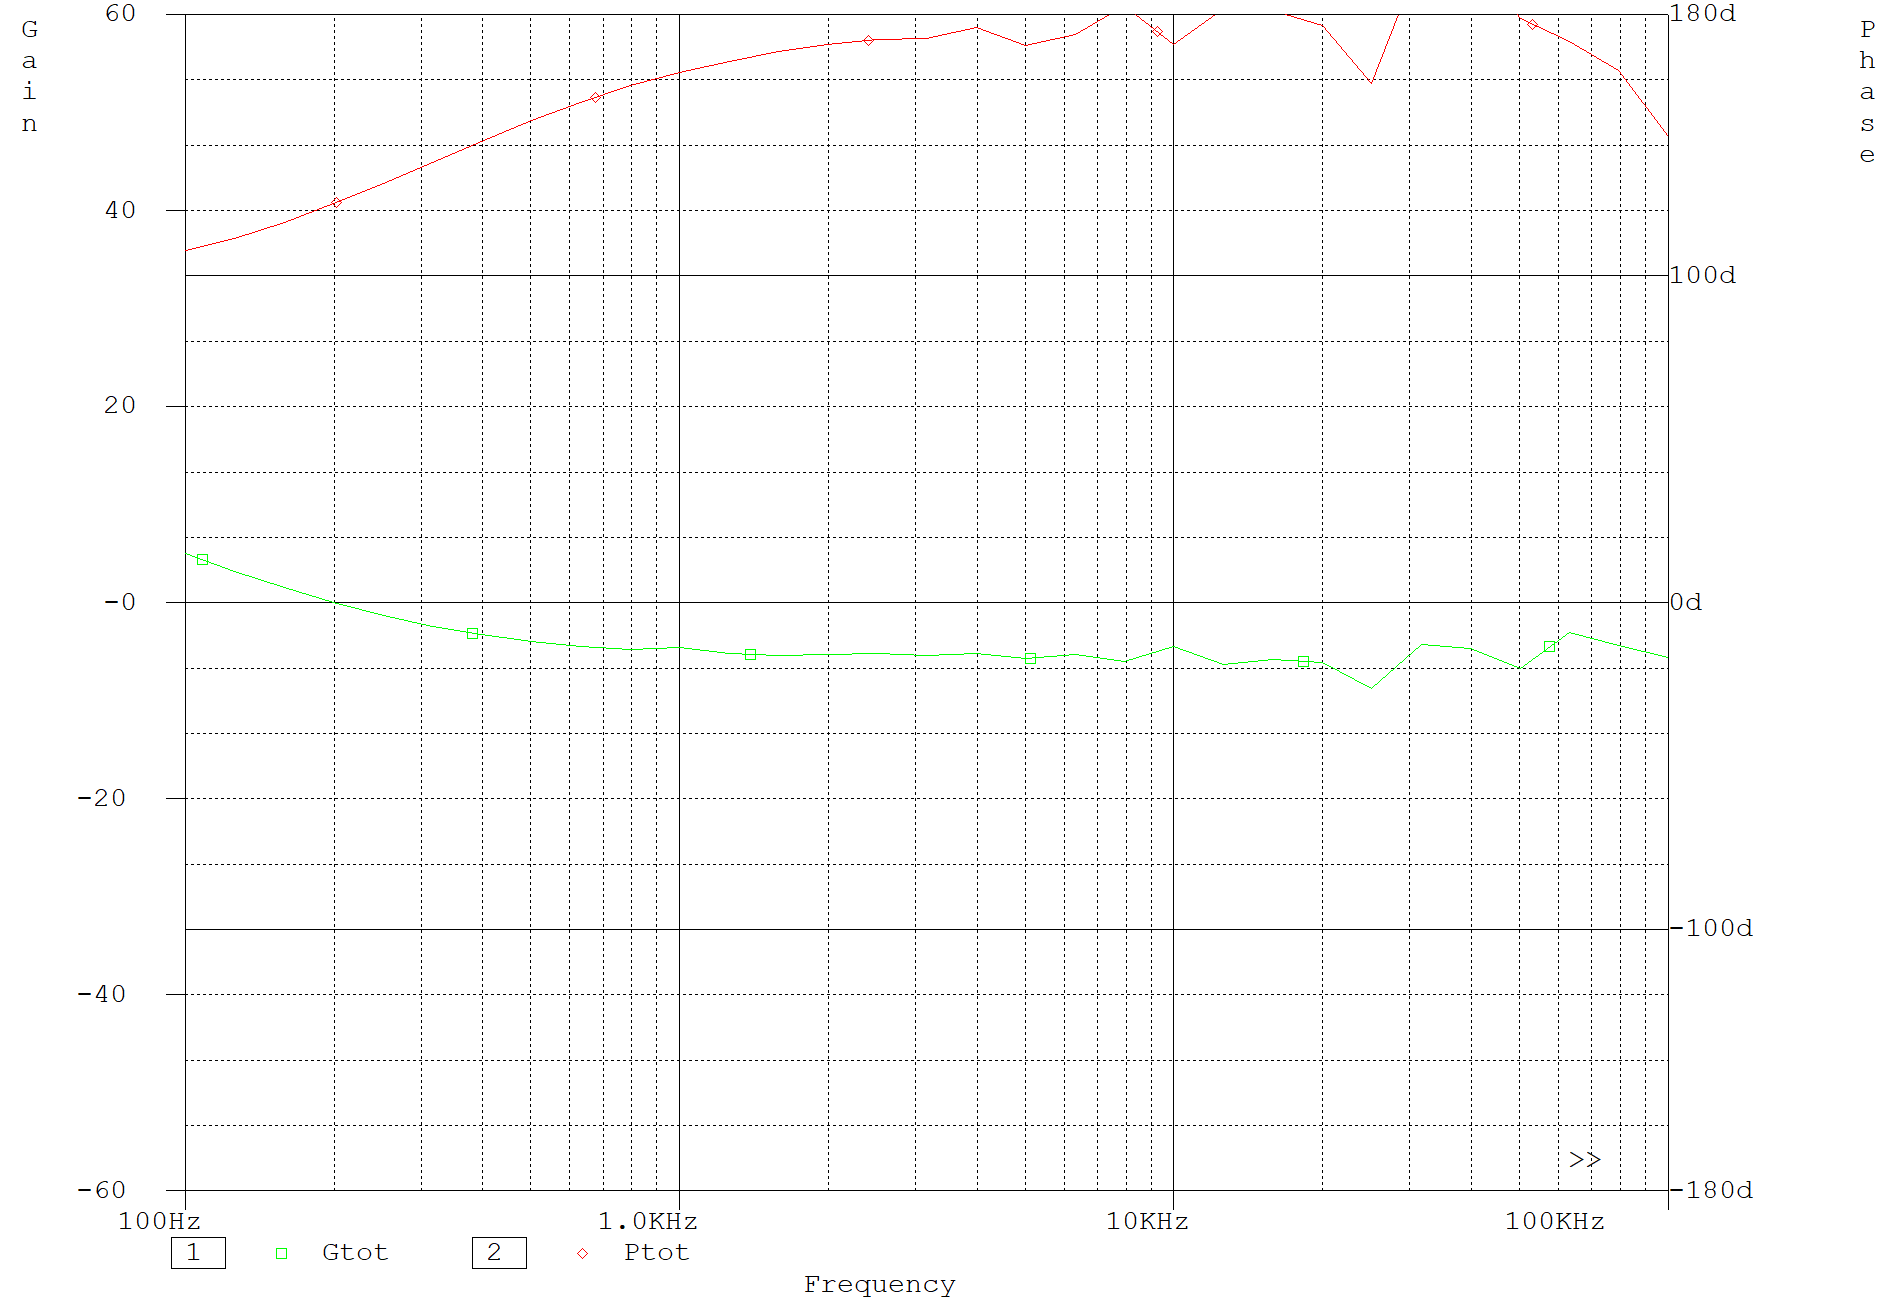
\includegraphics[max width=0.7\linewidth]{/tex/2iteration/billeder/Simulering_gain_fase_2iteration_opamp.png}
	\caption{Gain-fase simulering for fejlforstærker}
	\label{fig:sim_gain_fase_2iteration_opamp}
\end{figure}


\noindent Simuleringen af gain-fase for det samlede system er vist på figur~\ref{fig:sim_gain_fase_2iteration_tot}. Der er målt over den modstand hvor fejlsignalet indføres. Det svarer også til indgangen af spændingsdeleren og udgangen af converteren. Her ses det samme, som ved power modulet, at simuleringen ved de høje frekvenser bliver usikker. Indførelsen af fejlforstærkeren ses, ved båndbredden er blevet begrænset til ca. $700\hertz$. Der er designet efter en båndbredde på ca. $800\hertz$. Gain-marginen kan ikke rigtig aflæses her, da simuleringen bliver ustabil inden fasen krydser $0^\circ$. Til gengæld kan fase-marginen aflæses til ca. $75^\circ$, hvilket i analysen blev designet til $74.3^\circ$. 

\begin{figure}[H]
	\center
	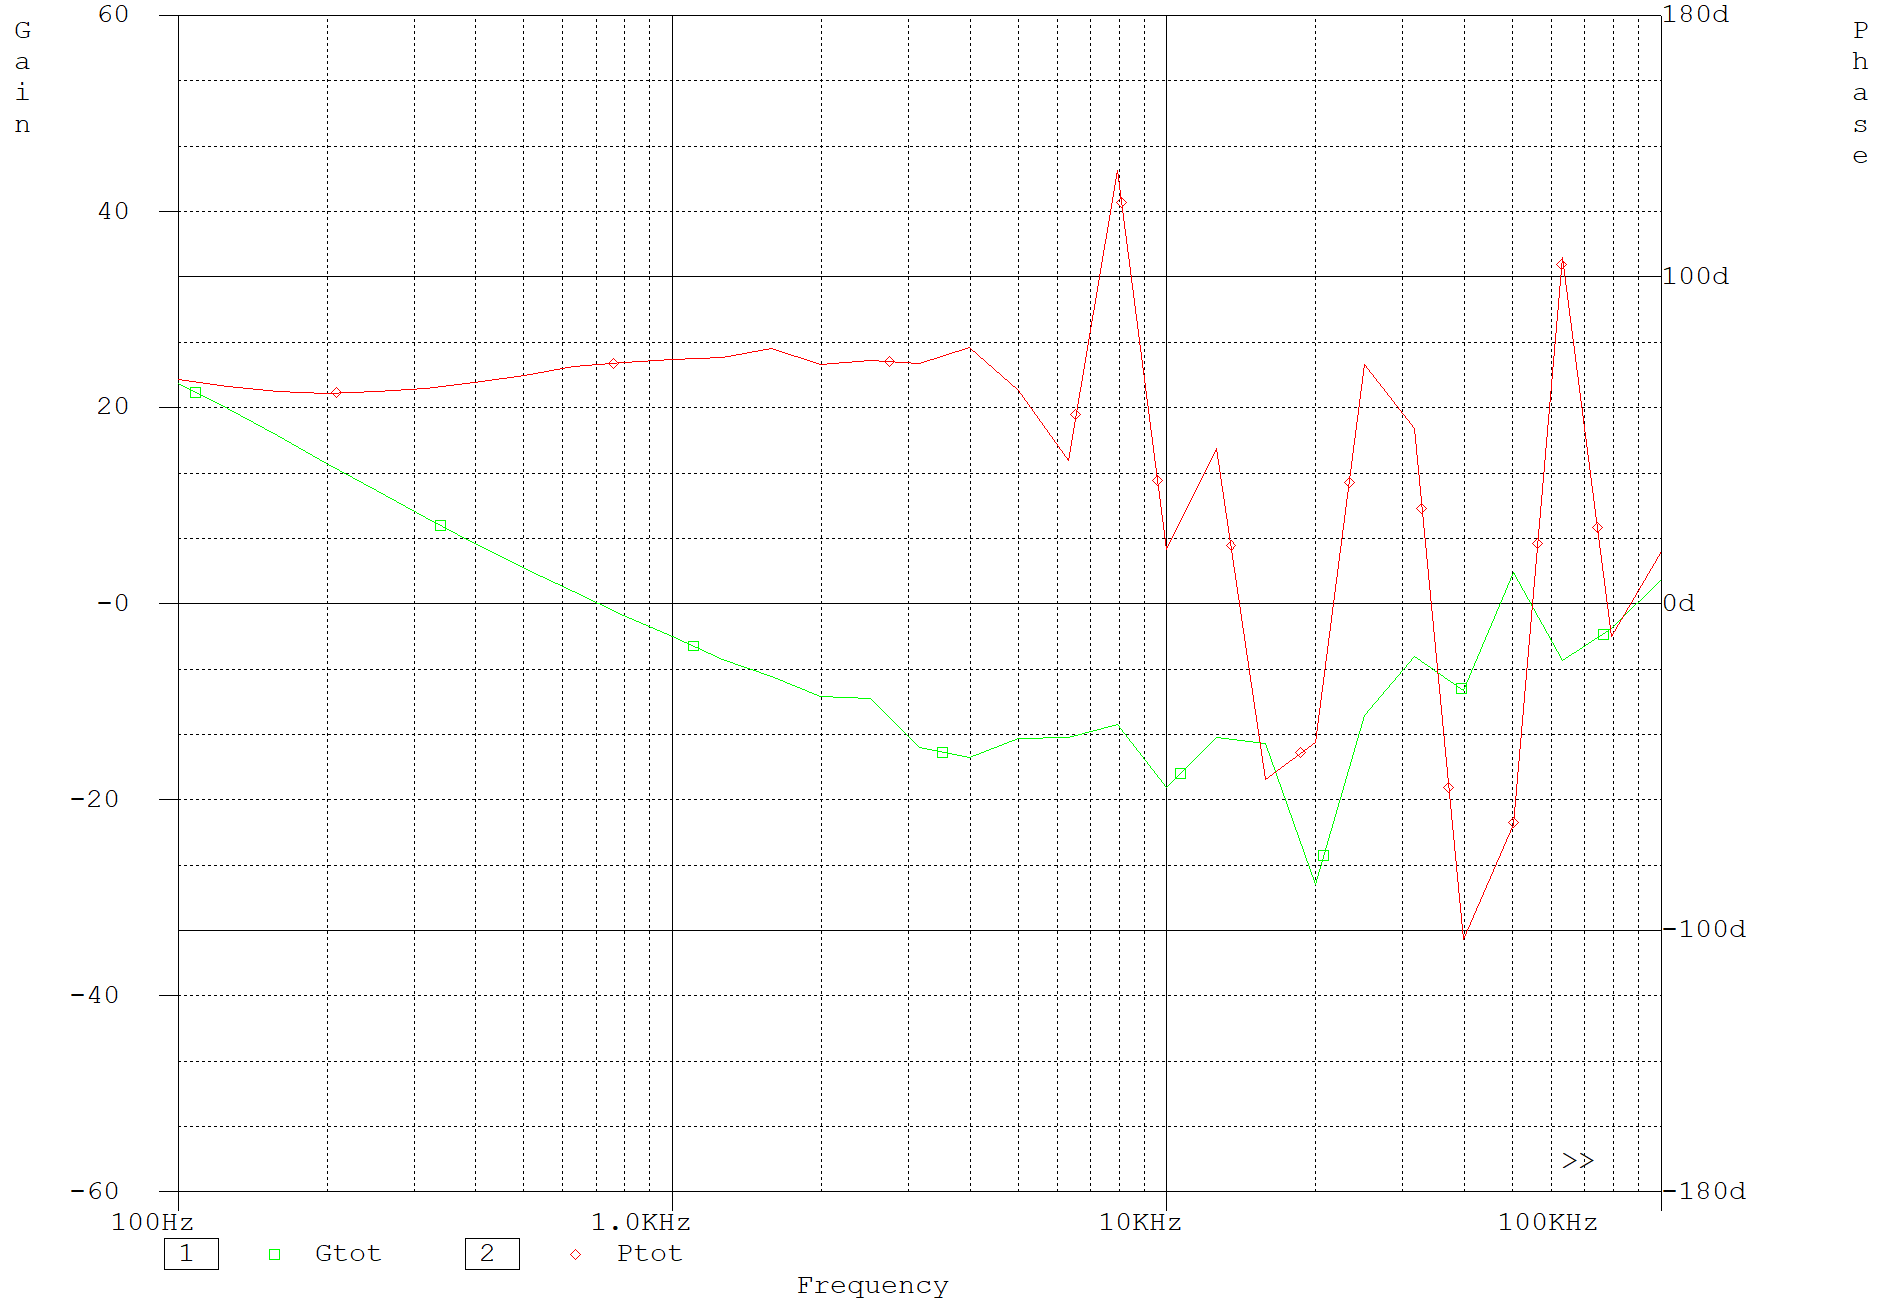
\includegraphics[max width=0.7\linewidth]{/tex/2iteration/billeder/Simulering_gain_fase_2iteration_tot.png}
	\caption{Gain-fase simulering for det samlede system}
	\label{fig:sim_gain_fase_2iteration_tot}
\end{figure}




